%%=============================================================================
%% Lesvoorbereiding
%%=============================================================================

\chapter{\IfLanguageName{dutch}{Lesvoorbereiding}{Lesson preparation}}
\label{ch:lesvoorbereiding}

Dit onderdeel van het onderzoek bestaat uit een lesvoorbereiding van het besproken raadspel. Dit bestaat uit een inleiding, een probleemstelling, een uitwerking en conclusie. Deze lesvoorbereiding werd verstuurd naar verschillende leerkrachten in de eerste graad secundair onderwijs. Deze leerkrachten hebben al ervaring met het implementeren van computationeel denken in hun lessen. Er werd hun gevraagd of de lesvoorbereiding zou werken in de praktijk (in een echte les). 

\section{Document}

\subsection{Inleiding en voorwoord}
Ik wil u persoonlijk bedanken voor uw interesse in mijn bachelorproef. Uw feedback op dit project zal een grote bijdrage leveren aan mijn onderzoek. Op het einde van dit document vraag ik u om uw feedback. Als u en uw feedback wenst anoniem te blijven in mijn paper, is dit zeker mogelijk, op aanvraag.

De bedoeling was om dit project uit te voeren in een klas. Spijtig genoeg, door de huidige covid-situatie en een tekort aan hardware, leek dit plan onrealistisch. Om dit project toch les-klaar te maken, heb ik besloten om een lesvoorbereiding te schrijven die de leerdoelen aangrijpt en het project uitlegt, stap per stap.

Dit document is onderdeel van mijn bachelorproef en bestaat uit een lesvoorbereiding voor een python project. Dit project wordt uitgevoerd op een Raspberry Pi, een minicomputer speciaal gemaakt om te leren programmeren. Dit project tackelt de eindtermen over Digitale Competentie en Media wijsheid, en specifieker de einddoelen van computationeel denken. Dit is geen erkende lesvoorbereiding en zou dus elementen kunnen missen.

Aan het einde van dit voorstel vraag ik u om uw feedback. Dit kan gaan van diepgaande feedback over de inhoud tot meer oppervlakkige kritiek. Op het einde vraag ik u of uw dit project realistisch vindt in een klassfeer en als u dit zelf zou willen uitvoeren met een Raspberry Pi. Deze feedback ontvang ik graag via mail: warre.vandeveire@gmail.com.

Nogmaals bedankt voor uw interesse en tijd,
Warre Van de Veire

\subsection{Overzicht van project}
Dit project bestaat uit het maken van een Python applicatie die een getal kan raden van een gebruiker. 
Zo moet de gebruiker bij de start van het spel een getal kiezen tussen 1 en 100. Hierna zal de computer een willekeurig getal presenteren. De gebruiker moet hierop feedback geven. Zo kan de gebruiker kiezen tussen drie opties: hoger, lager of correct. Wanneer de gebruiker hoger of lager ingeeft, zal de computer de feedback toepassen en een nieuwe gok wagen. Wanneer de gebruiker “correct” ingeeft, stopt het spel en presenteert de computer het correct geraden getal.

Dit project maakt gebruik van de Python programmeertaal en een Raspberry Pi. In de bijlage van deze lesvoorbereiding zit een beschrijving van de Raspberry Pi en de programmeertaal in kwestie. 
Dit document bestaat uit een introductie op het project, de probleemstelling, de uitwerking en een conclusie. Deze stappen zijn noodzakelijk voor het slagen van mijn onderzoek en de verwerking ervan in een klassfeer. 

\subsection{Uitdagingen}
\begin{itemize}
    \item Gebruik van de text-based programmeertaal: Python
    \item Gebruik van basis-instructies:
    \subitem Een lus
    \subitem Een voorwaarde
    \subitem een sequentie
    \subitem Gebruikersinput
    \item Gebruik van de Raspberry Pi
\end{itemize}

\subsection{Doelstellingen}
\begin{itemize}
    \item Verwerven van de competenties rond computationeel denken
\end{itemize}

\subsection{Voorkennis}
\begin{itemize}
    \item Basisinstructies van Python
    \subitem 'If'-voorwaarde
    \subitem 'While'-voorwaarde
    \subitem Variabelen
    \subitem Input
\end{itemize}

\subsection{Vereisten/taken}
\begin{enumerate}
    \item Alle onderdelen van computationeel denken moeten duidelijk aanwezig zijn in het project:
    \subitem Decompositie
    \subitem Abstractie
    \subitem Patroonherkenning
    \subitem Algoritmes
    \item Er mag zo weinig mogelijk gebruik gemaakt van vaktermen. Zo moet dit project uitvoerbaar blijven voor leerkrachten met een minimum aan programmeerkennis.
    \item De stappen voor het uitwerken van deze opdracht moeten duidelijk uitgelegd worden, waardoor er weinig nood is externe hulp.
    \item Het project moet uitvoerbaar zijn op een Raspberry Pi en moet de programmeertaal Python gebruiken.
    \item Het uitvoeren van het project mag niet langer dan twee lesuren duren: 2x50min.
    \item Het project moet een creatieve ingeving hebben en moet interessant blijven voor de leerlingen van de eerste graad.
\end{enumerate}

\subsection{Uitwerking}
\subsubsection{Introductie van het project}
\emph{Om het project te introduceren, lijkt het goed om luchtig te starten. We moeten dit ook kunnen terugkoppelen naar een probleem in de realiteit. Zo kunnen we gebruik maken van de eigenschappen van computationeel denken om aan te tonen dat dit vaak in de realiteit, onbewust, wordt gebruikt.}

Start de les met het spelen van het raadspel, zonder gebruik te maken van de computer. De leerkracht kan oftewel zelf een getal proberen te raden van een student of omgekeerd. De bedoeling is dat de leerling een idee krijgt hoe het spel werkt. 

Na een paar keer te spelen, zal de leerkracht opnieuw het spel uitvoeren, maar nu met behulp van het uitgewerkte project. Zo moet een leerling een getal verzinnen tussen 1 en 100 en moet de computer het raden. Nu de leerling het spel snapt en het uitgewerkte project in actie heeft gezien, kunnen we verdergaan naar de probleemstelling.

\subsubsection{Probleemstelling}
\emph{In dit onderdeel zullen we bespreken wat we precies willen bereiken en hoe we dit kunnen aanpakken. Hierin maken we gebruik van decompositie om de opdracht op te delen in kleinere, sub problemen. Hierna kunnen we, dankzij abstractie, deze kleinere problemen versimpelen. Dankzij patroonherkenning kunnen we deze problemen omvormen naar gelijkaardige oplossingen. Na we alle stappen hebben aangehaald, kunnen we deze stappen op een logische manier sorteren en gieten in een algoritme. Hiermee is het probleem opgelost en hebben we ons project gemaakt.}

We kunnen het gehele spel onderverdelen in verschillende, kleinere problemen. We starten bij het identificeren van de rollen. Probeer hiermee af te vragen wie er speelt. Zo kan de speler een groep leerlingen zijn of een enkele. We proberen dit echter simpel te houden, dus kiezen we voor één gebruiker.

\underline{Vragen:}
\begin{itemize}
    \item Wie speelt het spel?
    \item Welke partijen zijn hierbij betrokken?
\end{itemize}
\underline{Oplossing:}
\begin{itemize}
    \item Rol 1: De speler $\rightarrow$ leerling
    \item Rol 2: De rader $\rightarrow$ computer
\end{itemize}

Nu we de rollen hebben geïdentificeerd, kunnen we bekijken wat elke rol precies uitvoert. Som alle acties op die de rollen uitvoeren bij het maken van dit project. Plaats deze acties onder de rol.

\underline{Vragen:}
\begin{itemize}
    \item Welke acties voeren deze rollen uit doorheen het spel?
    \item Communiceren deze rollen met elkaar?
\end{itemize}
\underline{Oplossing:}
Zie figuur \ref{fig:lesvoor_prob1}

\begin{figure}
    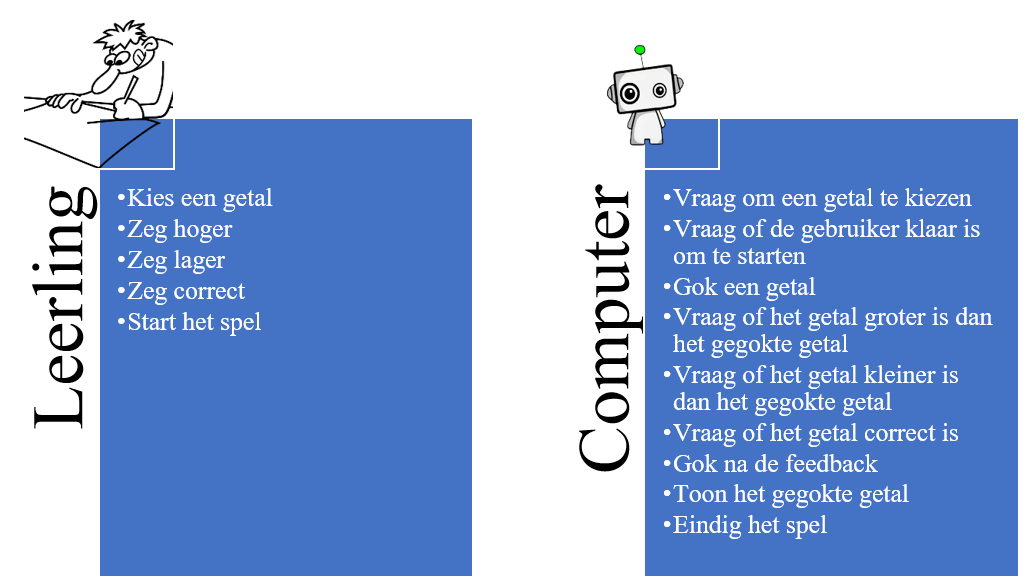
\includegraphics[width=\linewidth]{probleemstelling1}
    \caption{Alle acties per rol}
    \label{fig:lesvoor_prob1}
\end{figure}

Nu we de rollen duidelijk kennen en de acties die worden uitgevoerd, kunnen we deze problemen versimpelen door bepaalde acties onder een noemer te plaatsen. Aangezien de computer de meeste taken heeft, zal er vooral bij deze rol versimpelt moeten worden. Dit maakt het project makkelijker te begrijpen en haalt de complexiteit ervan weg. Dankzij abstractie kunnen we bijvoorbeeld bepaalde taken groeperen onder één actie.

\underline{Vragen:}
\begin{itemize}
    \item Welke acties kunnen we groeperen?
    \item Welke acties kunnen we tegelijkertijd uitvoeren doorheen het spel?
    \item Welke acties zijn noodzakelijk voor het uitvoeren van het spel en welke kunnen we weglaten?
\end{itemize}
\underline{Oplossing:}
Zie figuur \ref{fig:lesvoor_prob2}

\begin{figure}
    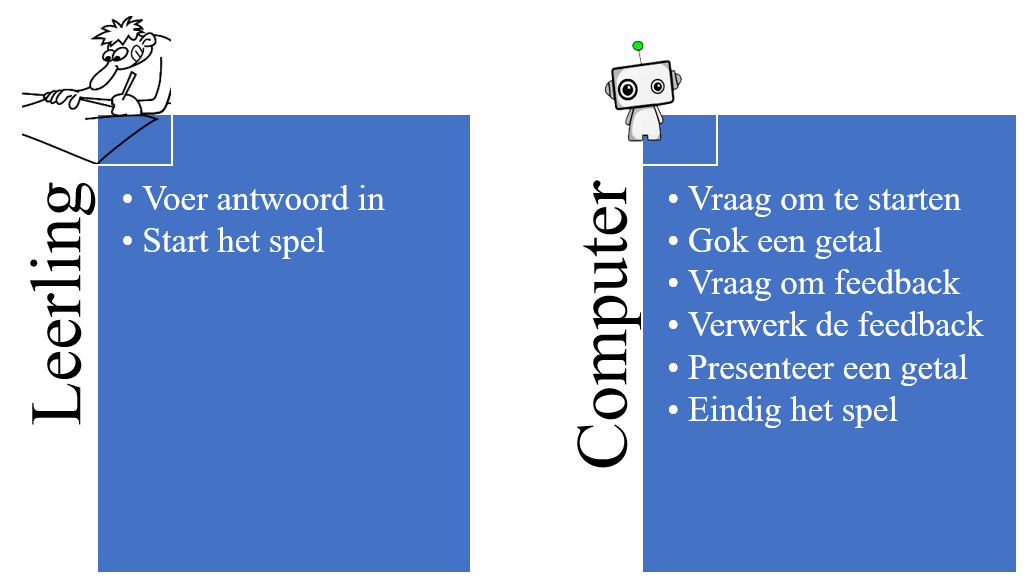
\includegraphics[width=\linewidth]{probleemstelling2}
    \caption{Alle versimpelde acties per rol}
    \label{fig:lesvoor_prob2}
\end{figure}

Nu we duidelijk de rollen en de acties hebben opgesomd, kunnen we alles in een logische volgorde gieten. Maak een schema op met de logische volgorde. Zet hierbij ook de juiste instructies om zo de link met Python makkelijker te maken. Met patroonherkenning kunnen we bijvoorbeeld inzien dat we werken met een lus van onbepaalde duur.

\underline{Vragen:}
\begin{itemize}
    \item Welke acties volgen elkaar op?
    \item Welke acties worden herhaald?
    \item Moet een rol wachten op de actie van een andere rol?
    \item Zijn er acties die tegelijk lopen?
    \item Welke acties hebben invloed op elkaar?
\end{itemize}
\underline{Oplossing:}
Zie figuur \ref{fig:lesvoor_prob3}

\begin{figure}
    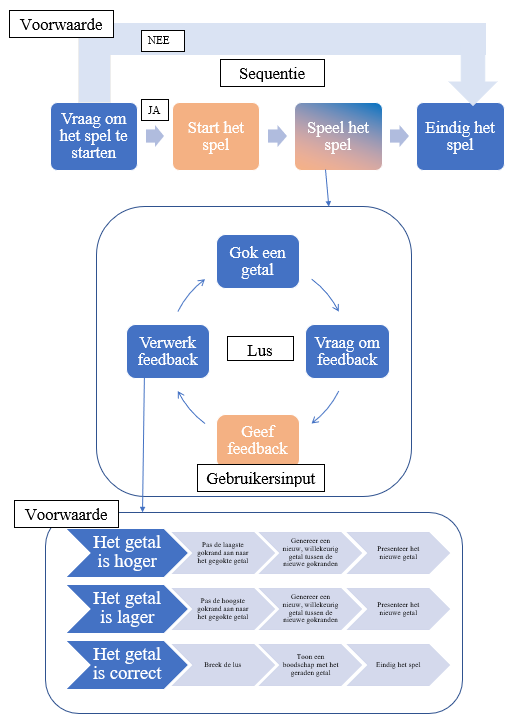
\includegraphics[width=\linewidth]{probleemstelling3}
    \caption{Uitgewerkt overzicht met alle acties, op logische volgorde}
    \label{fig:lesvoor_prob3}
\end{figure}

Dankzij de eigenschappen van computationeel denken hebben we nu een simpel raadspel opgedeeld en uitgewerkt. Nu we weten wat er precies uitgevoerd moet worden, kunnen we starten met het uitwerken van dit spel in Python.

\subsubsection{Uitwerking}
\emph{We zullen het proces, uitgewerkt in de probleemstelling, nu maken in Python. Hiervoor maken we gebruik van een Raspberry Pi als computer en Thonny als IDE. Thonny is een beginnersvriendelijke ontwikkelomgeving speciaal ontworpen voor de Raspberry Pi. We gaan elke stap in de probleemstelling omvormen naar Python code om een werkende applicatie te bekomen. In figuur \ref{fig:lesvoor_rasp1} en figuur \ref{fig:lesvoor_rasp2} kunt u zien hoe u Thonny gebruikt op een Raspberry Pi:}

\begin{figure}
    
\includegraphics[width=\linewidth]{lesvoorbereidingPi1}
    \caption{Opstartscherm van de Raspberry Pi OS}
    \label{fig:lesvoor_rasp1}
\end{figure}

\begin{figure}
    
\includegraphics[width=\linewidth]{lesvoorbereidingPi2}
    \caption{Openen van Thonny via het startmenu}
    \label{fig:lesvoor_rasp2}
\end{figure}

We starten eerst met de opbouw van de Python applicatie. Dit begint bij het maken van een methode en dan hierop verder te bouwen. We starten vanuit de sequentie en gaan zo dieper in de applicatie. 

\emph{Bij het starten van Thonny krijgt u dit scherm te zien (zie figuur \ref{fig:uitwerking1} ):
    U ziet direct twee schermen: het script scherm en de shell. In het script scherm zullen de leerlingen hun code schrijven. Dankzij de shell zullen de leerlingen het spel kunnen spelen.}

\begin{figure}
    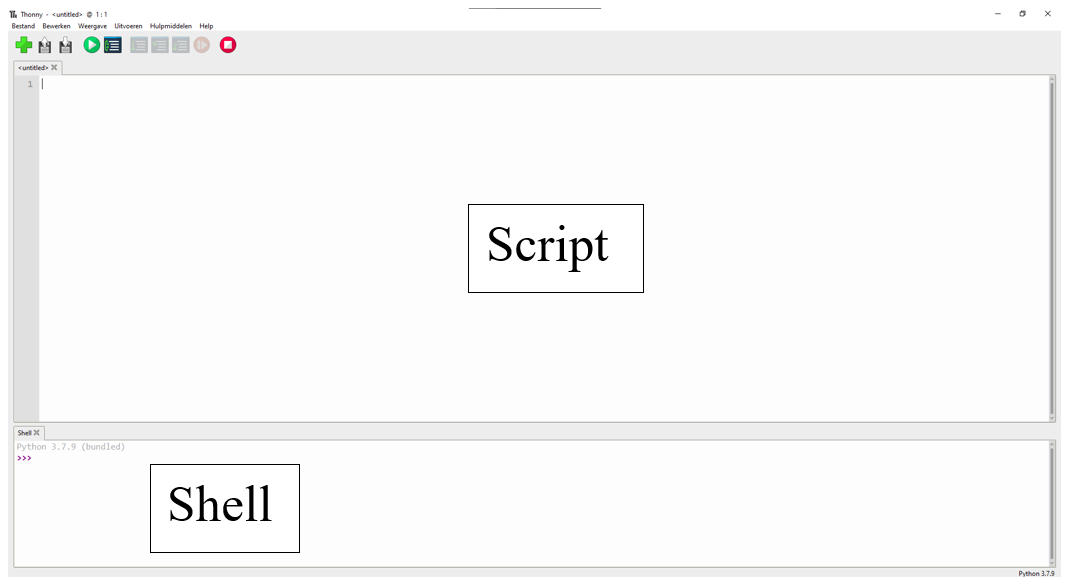
\includegraphics[width=\linewidth]{uitwerking1}
    \caption{Thonny startscherm}
    \label{fig:uitwerking1}
\end{figure}

Het volledige uitgewerkte project zal er uiteindelijk zo uit zien (zie figuur \ref{fig:uitwerkingAfgewerkt}).

\begin{figure}
    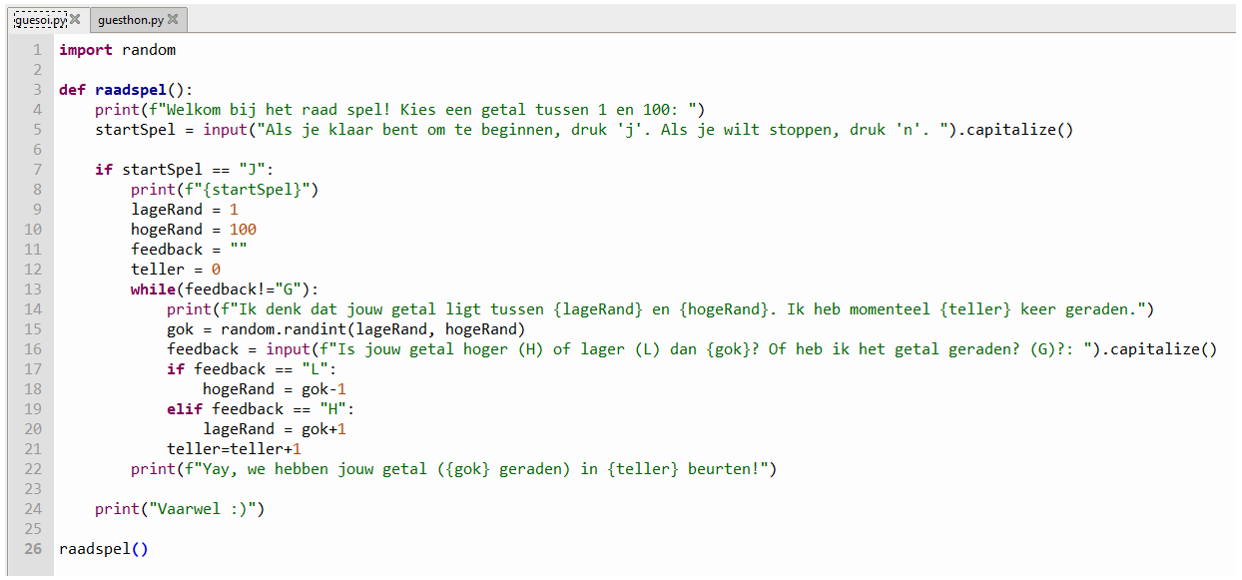
\includegraphics[width=\linewidth]{uitgewerkt}
    \caption{Het uitgewerkte raadspel}
    \label{fig:uitwerkingAfgewerkt}
\end{figure}

\underline{De sequentie + voorwaarde}

We zullen eerst de hoofdsequentie omvormen. Deze start de applicatie spel, vraagt om een input en stopt het spel.

We hebben dus nood aan een inputwaarde. In Python wordt dit gedefinieerd door een variabele gelijk te stellen aan een input methode. We geven in de haakjes van de input een boodschap mee die de gebruiker uitlegt wat te doen (zie figuur \ref{fig:uitwerking2}):

\begin{figure}
    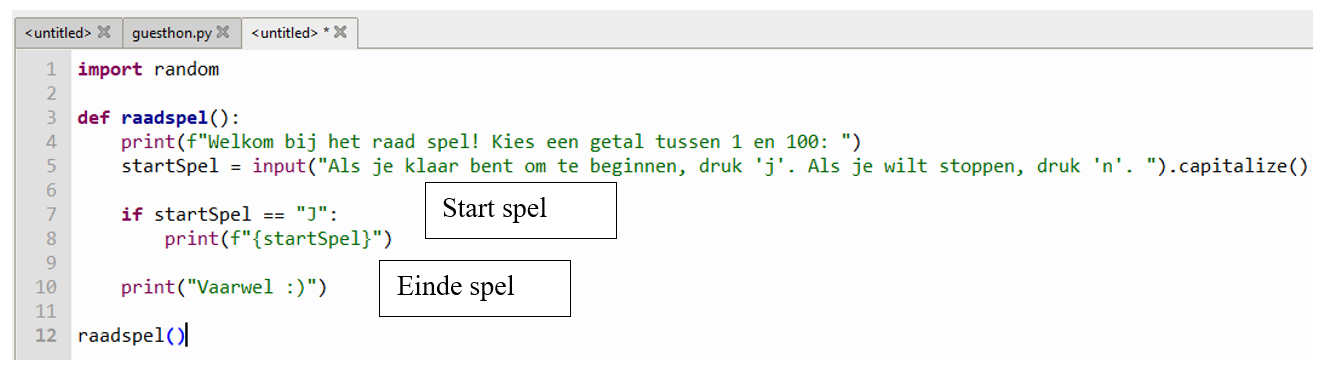
\includegraphics[width=\linewidth]{uitwerking2}
    \caption{Eerste stap uitgewerkt: sequentie + voorwaarde}
    \label{fig:uitwerking2}
\end{figure}

\textbf{UITBREIDING}: Dankzij de 'capitalize()'-methode, zal de input omgezet worden naar hoofdletters. Dit zorgt ervoor dat de gebruiker zowel een kleine letter 'j' als grote letter 'J' kan ingeven, aangezien het allemaal omgezet wordt naar grote letters.

Dankzij de 'if'-instructie kunnen we een voorwaarde toevoegen. Bij deze voorwaarde bekijkt hij als de input gelijk is aan 'J'. 
Dankzij de print('…') methode kunnen we een melding weegeven.

\textbf{UITBREIDING}: Je kan ook de waarde van 'startSpel' weergeven. Hierbij zetten we een f voor de aanhalingstekens en zetten we de waarde omringt door gekrulde haakjes. 

Wanneer de gebruiker nu 'J' ingeeft, ziet hij de input. Wanneer hij een andere letter ingeeft, stopt het spel.

\underline{De lus}

Nu we het spel kunnen starten, zullen we beginnen met het implementeren van de lus. De computer gaat constant vragen om feedback tot het getal geraden is. Hij zal dus bepaalde stukken code herhalen voor een onbepaalde duur: we weten op voorhand niet hoeveel keer de computer zal nodig hebben om het getal te raden.  

In de voorwaarde zullen we nu een lus toevoegen. Eerst hebben we nood aan variabelen die onze zoekranden bijhoudt. Er is nood aan een hoge en lage rand. 
Er is ook nood aan een feedback variabele. Hierin zal de gebruiker dus zijn antwoord kunnen meegeven.
Tenslotte kunnen we een teller toevoegen die controleert hoeveel pogingen de computer nodig had om het getal te raden. Zie figuur \ref{fig:uitwerking3}:

\begin{figure}
    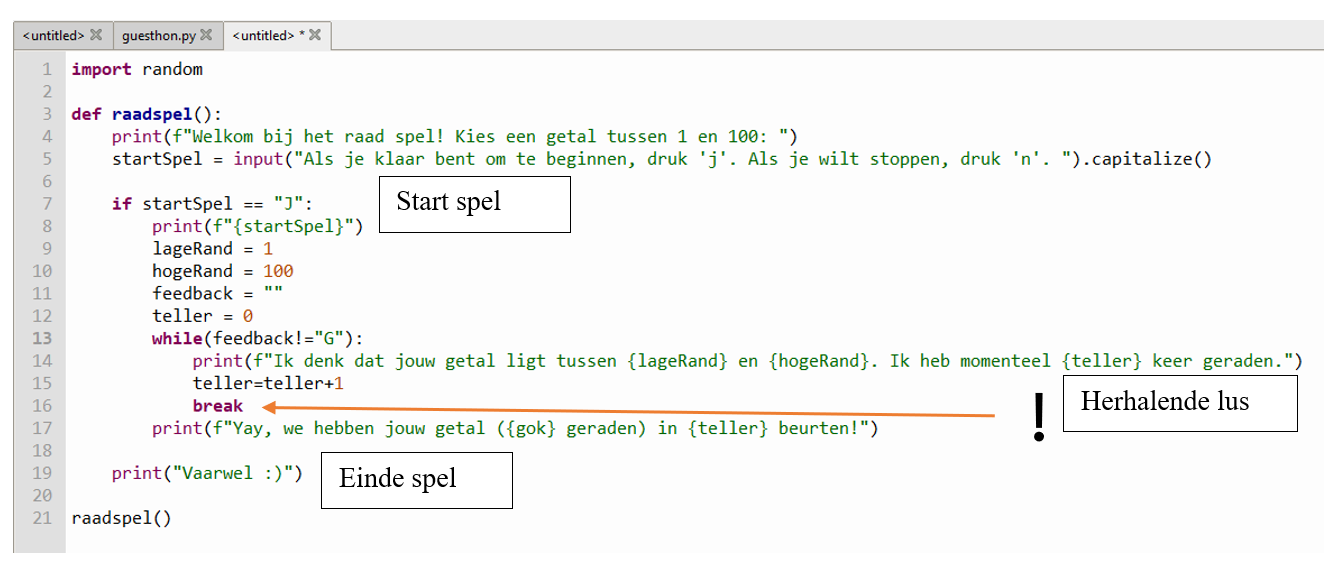
\includegraphics[width=\linewidth]{uitwerking3}
    \caption{Tweede stap uitgewerkt: de lus}
    \label{fig:uitwerking3}
\end{figure}

Zoals eerder vermeld gebruiken we een hoge en lage zoekrand. Deze zijn bij het begin van het zoeken 1 en 100, aangezien ons zoekveld ligt tussen deze waarden.
Het feedback veld blijft nu even leeg. We vragen nog niet aan de gebruiker als het getal hoger of lager ligt.
De teller heeft ook een standaardwaarde. Deze zal verhoogd worden bij elke lus.

Aangezien we niet weten hoe vaak de computer gaat proberen te raden, zullen we een 'while'-instructie gebruiken. Zolang de voorwaarde in de haakjes klopt, worden de instructies vanbinnen herhaald. 
Wanneer deze voorwaarde niet meer klopt, stopt de lus.
In ons geval zal de lus stoppen wanneer de variabele 'feedback' gelijk is aan 'G'. 
Met de syntax binnen de haakjes wordt dus verteld: 
zolang feedback NIET GELIJK AAN (!=) 'G' is, zal de lus opnieuw doorlopen worden.

\textbf{BELANGRIJK}: aangezien we momenteel de feedback niet aanpassen, zal deze lus in de oneindigheid blijven doorlopen. Het is dus belangrijk om een 'break' te plaatsen op het einde van de lus. Dit breekt sowieso de lus, los van de verklaring tussen de haakjes.

\underline{De gebruikersinput: gokken en het ingeven van feedback}
We hebben een lus die wacht op de feedback van de gebruiker. Nu moeten we dus feedback kunnen geven op een gok. We zullen dus de computer een variabele “gok” laten bijhouden die een willekeurige waarde tussen de zoekranden genereert (zie figuur \ref{fig:uitwerking4}):

\begin{figure}
    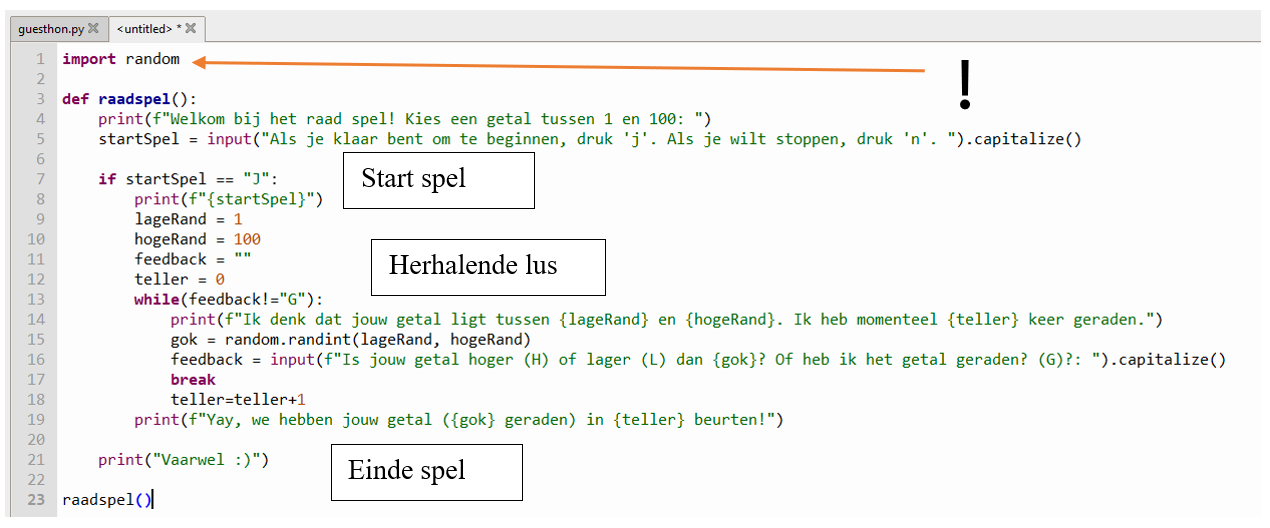
\includegraphics[width=\linewidth]{uitwerking4}
    \caption{Derde stap uitgewerkt: de gebruikersinput}
    \label{fig:uitwerking4}
\end{figure}

Zoals je kunt zien, de computer maakt een willekeurig getal aan dankzij de hoge en lage zoekrand. Dit doen we dankzij het geïmporteerde object: random. De methode 'randint' genereert dit willekeurig getal. Dankzij de argumenten tussen deze haakjes weet de methode randint() tussen welke waarden het getal moet gekozen worden.

Pas nadat de computer een gok heeft gemaakt, kan het vragen om feedback aan de gebruiker. We passen dus de waarde aan van feedback, dankzij een tweede input. Ook deze input zullen we in hoofdletters omvormen.

\underline{Geavanceerdere voorwaarden: feedback verwerken en zoekranden aanpassen}

We krijgen feedback binnen van de gebruiker. Deze kan oftewel hoger (H), lager (L) of geraden (G) antwoorden. Aangezien de lus zal beëindigd worden bij het invoeren van G, moeten we hiervoor geen voorwaarde schrijven. We moeten wel de zoekranden aanpassen wanneer de gebruiker hoger of lager ingeeft. Zie figuur \ref{fig:uitwerking5}:

\begin{figure}
    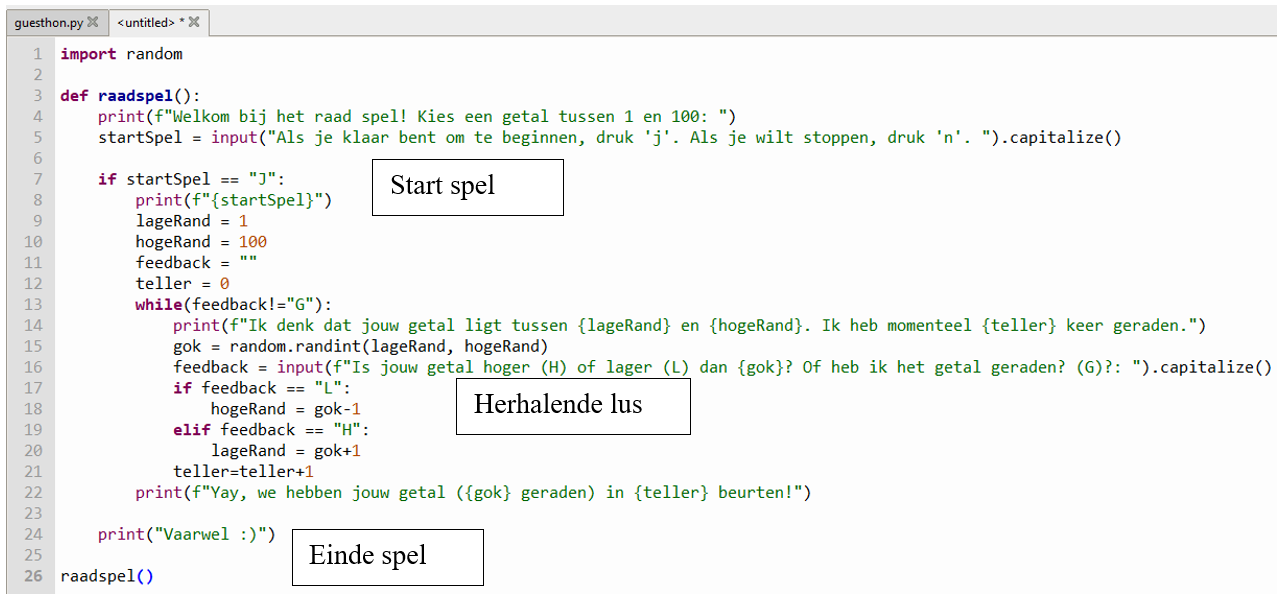
\includegraphics[width=\linewidth]{uitwerking5}
    \caption{Vierde stap uitgewerkt: Geavanceerde voorwaarden}
    \label{fig:uitwerking5}
\end{figure}

In dit geval maken we gebruik van een tweedelige voorwaarde. We bekijken eerst als de ingegeven feedback \emph{lager} was. Wanneer dit het geval is, passen we onze hoge zoekrand aan naar de gegokte waarde. Het te zoeken getal is nl. kleiner dan de huidige bovengrens (opgeslagen in de variabel \emph{hogeRand})
We trekken er nog één vanaf, aangezien we de gegokte waarde niet willen toevoegen in het zoekgebied.

Als de computer ziet dat de gebruiker geen 'L' heeft ingegeven, zal het bekijken als de feedback een 'H' is. Dit vind je terug in het tweede deel van de voorwaarde (elif). Als de echte waarde groter is dan de gegokte waarde, zal het de \emph{lage zoekrand} aanpassen. Ook dit keer willen we de gokwaarde niet opnemen in het zoekgebied.

Nu is ons raadspel zo goed als af. We moeten enkel nog een boodschap meegeven die ons vertelt dat het getal geraden is en in hoeveel beurten. Deze boodschap moet slechts 1 maal afgedrukt worden, aan het einde van het spel
We voegen daarom een print() methode uit BUITEN de lus.

En zo is het project afgewerkt. Als een leerling op de speel-knop drukt (groene pijl links-bovenaan, zie figuur \ref{fig:uitwerking1}), start het spel in de shell. Volg de instructies en laat de computer uw getal raden.

\emph{UITBREIDING}: Het spel werkt, maar is nog niet fout-vriendelijk. Als je per ongelijk een verkeerd antwoord ingeeft, is de kans groot dat het gekozen getal niet meer in het zoekgebied ligt. Ook zou het kunnen dat de hoge zoekrand lager komt te liggen dan de lage zoekrand. Dit zou het spel breken. Met het volgende stukje code toe te voegen, zou je dit probleem kunnen vermijden:

\begin{lstlisting}[language=Python, caption=Volledige uitwerking van het raadspel in Python]
if lageRand == hogeRand:
    gok = hogeRand
else:
    gok = random.randint(lageRand, hogeRand)
\end{lstlisting}

\subsubsection{Conclusie}
We hebben succesvol een raadspel kunnen maken in Python. Dankzij de eigenschappen van computationeel denken hebben we dit probleem makkelijk kunnen ontleden en omvormen naar leesbare code.

\subsection{Bedanking}
Ik bedank nogmaals uw interesse in mijn bachelorproef. Als u feedback zou hebben op dit document, stuur mij graag een bericht voor 28/05/2021 om 12u via warre.vandeveire@gmail.com 

Bedankt en nog een prettige dag.

\subsection{Bijlage}
\emph{\underline{Raspberry Pi:}} 
De Raspberry Pi is een single board computer: een volledige functionele computer op een enkele printplaat.
Opgericht in 2008 als liefdadigheidsinstelling in het Verenigd Koninkrijk, staat de Raspberry Pi Foundation in voor het verspreiden van computationele en digitale kennis over de hele wereld. Zo organiseert Raspberry verschillende workshops en events om het potentieel van de Raspberry Pi te demonstreren.
Ook moedigt Raspberry verschillende scholen over de hele wereld aan om gebruik te maken van hun technologie in de klas. Zo wil het niet alleen programmeren populair maken, maar wil het ook technologie introduceren in andere wetenschappelijk vakken zoals fysica of chemie.

\emph{\underline{Python:}}
Python is een klassieke text-based programmeertaal. De gebruiker schrijft zelf de instructies uit die de computer moet uitvoeren. Dit, in tegenstelling tot Scratch, is de meest gebruikte vorm van programmeren en is de norm in de professionele wereld. Python is een open-source codetaal: iedereen mag er gratis gebruik van maken, zonder te betalen.
Dit is niet zo abnormaal in de wereld van codetalen. Wat Python uniek maak, is zijn lage complexiteit. In tegenstelling tot bekende programmeertalen zoals Java, is gemakkelijk te lezen en is de instap veel lager.


\section{Feedback}
Zoals eerder vermeld, werd deze lesvoorbereiding verstuurd naar verschillende leerkrachten in de hoop om hun feedback te ontvangen.
De belangrijkste vragen waren als volgt:
\begin{itemize}
    \item Vind u deze les realistisch in een les in de eerste graad?
    \item Zou u het zien zitten om dit project uit te werken met behulp van een Raspberry Pi en Python?
\end{itemize}
Na het ontvangen van een aantal kritische kijken kunnen we evalueren als ons onderzoek zou slagen in de praktijk. 

De algemene consensus was dat het project interessant lijkt en zeker leuk om uit te voeren in de les. Ook was de lesvoorbereiding goed opgesteld en werden de eigenschappen van computationeel denken duidelijk uitgewerkt. Tenslotte leek het werken met een Raspberry Pi een interessante uitdaging. 

Het probleem viel bij de meeste leerkrachten bij de keuze van programmeertaal, namelijk Python.
Volgens Sean Callens\footnote{Leerkracht informatica bij Atheneum Voskenslaan} ligt het probleem vooral bij de syntax-kennis. Om Python correct te kunnen gebruiken, heb je nood aan een voorkennis over de specifieke syntax. Dit zou in de praktijk een te groot obstakel kunnen vormen voor leerlingen van de eerste graad. Callens stelt dus voor om dit eerder te organiseren in een tweede graad. Scratch zou, volgens Callens, een veel intuïtievere programmeertaal zijn. Hierbij kan er nadruk gelegd worden op het probleemoplossend gedeelte van programmeren, zonder de leerlingen te belasten met syntax-kennis en foutbestendigheid. 

Ook volgens Lieve Van Bastelaere\footnote{leerkracht bij VTI Puytenput} zal Python het grootste obstakel vormen. Volgens haar ligt het probleem meer met het niveau van Engels in de eerste graad. Er wordt meer gewerkt met de scratchomgeving. Deze is een stuk gebruiksvriendelijker dan de pythonomgeving. Volgens Van Bastelaere wordt momenteel vooral gewerkt met trail-and-error opgaves om te leren programmeren. Scratch is hiervoor optimaal, aangezien het 'bugs' en fouten in de code zelf opvangt. Bij Python moet je al een idee hebben hoe je een fout kan lezen, laat staan te fixen. Met al deze factoren zou het moeilijk zijn voor de studenten om de aandacht erbij te houden.


We kunnen dus concluderen uit de feedback dat vooral de keuze in programmeertaal een probleem zal vormen. de python-syntax zal te moeilijk zijn voor kinderen van de eerste graad om te begrijpen. Om de trail-and-error methode te gebruiken om te leren programmeren, moet de programmeertaal zelf al veel fouten moeten kunnen tegenhouden. Python is hiervoor niet ontworpen. Ze zouden al een foutmelding krijgen van een kleine tikfout.